% Engine: pdfLaTeX. Proposed results for coauthor review, not a submission.
\documentclass[10pt,letterpaper]{article}
\usepackage[T1]{fontenc}
\usepackage{lmodern}
\usepackage[margin=0.8in]{geometry}
\usepackage{amsmath,amssymb,amsthm,booktabs,graphicx,microtype}
\usepackage{enumitem}
\usepackage[dvipsnames]{xcolor}
\usepackage[colorlinks=true,linkcolor=MidnightBlue,urlcolor=MidnightBlue,citecolor=MidnightBlue]{hyperref}
\newtheorem{theorem}{Proposed theorem}
\newtheorem{corollary}[theorem]{Corollary}
\newcommand{\R}{\mathbb R}
\newcommand{\co}{\operatorname{conv}}
\newcommand{\dd}{\,\mathrm d}
\newcommand{\negorth}{\R^m_{\leq0}}
\setlength{\parskip}{4pt}
\setlength{\parindent}{0pt}
\setlist[itemize]{leftmargin=*,nosep}
\setlist[enumerate]{leftmargin=*,nosep}
\title{When More Functions Cannot Help:\\Moment Obstructions and Exact Degree Gaps\\for Discrete-Time Safety Certificates}
\author{Technical note prepared for Reza Iraji and Majid Zamani}
\date{October 5, 2026 --- research draft for coauthor review}
\begin{document}
\maketitle
\vspace{-1em}
\textbf{Research question.} At a prescribed polynomial degree, is failure of safety-certificate synthesis caused by insufficient functions, or by the global constant-comparison condition itself? Can the latter be diagnosed without choosing the number of functions or the comparison matrix?

\textbf{Answer developed here.} Constant comparisons are equivalent, under explicit regularity assumptions, to preservation of the nonpositive orthant by a \emph{convexified certificate-value transition relation}. A truncated-moment witness then rules out every fixed-anchor VBC at a specified degree. An exact polynomial example has minimum implication-IBC degree two and minimum constant-comparison fixed-anchor VBC degree four, allowing arbitrary finite component counts and either propagation direction.

\section{Definitions and a characterization for a fixed vector}
Retain the submitted paper's autonomous system $x^+=f(x)$, nonempty disjoint $X_0,X_u\subseteq X\subseteq\R^n$, and $f(X)\subseteq X$. A forward strict-margin fixed-anchor VBC is $B=(B_1,\ldots,B_m)^\top$ and a constant entrywise nonnegative $A$ satisfying
\begin{equation}\label{eq:vbc}
 B\leq-\delta_0\mathbf1\ \text{on }X_0,\qquad B_1\geq\delta_u\ \text{on }X_u,\qquad B(f(x))\leq AB(x)\ \text{on }X,
\end{equation}
where $\delta_0,\delta_u>0$. The backward definition reverses the separation sets and uses $B(x)\leq AB(f(x))$. A forward implication IBC has frames $b_i$, $b_1\leq0$ on $X_0$, every $b_i>0$ on $X_u$, and $b_i(x)\leq0\Rightarrow b_{\min\{i+1,m\}}(f(x))\leq0$ on $X$. A single frame is permitted. No bound on $\rho(A)$ is imposed. All degree bounds are total polynomial degree, including constants.

\begin{theorem}[Global comparison versus convexified invariance]\label{th:comparison}
Assume additionally that $X$ is compact, $f$ and $B$ are continuous, and some $x_*\in X$ satisfies $B(x_*)<0$ componentwise. Define
\[
 Q_B=\co\{(B(x),B(f(x))):x\in X\}\subseteq\R^{2m}.
\]
The following are equivalent:
\begin{enumerate}
\item There exists a constant $A\geq0$ with $B(f(x))\leq AB(x)$ throughout $X$.
\item Every $(s,t)\in Q_B$ with $s\leq0$ satisfies $t\leq0$.
\item For every probability measure $\mu$ on $X$, $\int B\dd\mu\leq0$ implies $\int B\circ f\dd\mu\leq0$.
\end{enumerate}
If no such $A$ exists, a violating measure can be chosen with at most $m+2$ atoms.
\end{theorem}
\begin{proof}
The inequality $t\leq As$ is affine and therefore persists on $Q_B$; $A\geq0$ gives (1)$\Rightarrow$(2). Compactness makes $Q_B$ compact, and its elements are exactly the barycenters of the transition-value graph, giving (2)$\Leftrightarrow$(3). For each row $i$, maximize $t_i$ over $Q_B$ subject to $s\leq0$. Under (2) its value $p_i\leq0$. The point induced by $x_*$ is strictly feasible; mixing it slightly with a relative-interior point gives strict feasibility in the affine hull. Finite-dimensional convex duality, applied on the affine hull of $Q_B$, gives an attained multiplier $a_i\geq0$ with
\[
 \max_{(s,t)\in Q_B}(t_i-a_i^\top s)=p_i\leq0.
\]
These row multipliers form $A$. If (2) fails in row $i$, apply Caratheodory's theorem to the projected graph $(B(x),B_i(f(x)))\in\R^{m+1}$ to obtain at most $m+2$ atoms.
\end{proof}

\newpage
\section{A degree obstruction independent of component count}
Theorem~\ref{th:comparison} distinguishes ordinary invariance of $S=\{B\leq0\}$ from the extra requirement: preservation of the orthant after mixing \emph{transition values}, even if the mixture is not induced by one state. It supplies the following useful sufficient regime. If $X$ is convex, every $B_j$ is convex and every $B_i\circ f$ is concave, ordinary invariance implies condition (3): Jensen's inequalities give $B(\bar x)\leq\int B\dd\mu\leq0$ and $\int B_i\circ f\dd\mu\leq B_i(f(\bar x))\leq0$. With the theorem's other assumptions, a constant comparison matrix therefore exists. These are sufficient conditions, not necessary ones.

Let $v_d(x)$ contain all monomials of total degree at most $d$, including $1$; its dimension is $N=\binom{n+d}{d}$. Write $M_d(\mu)=\int v_d\dd\mu$.
\begin{theorem}[Truncated-moment obstruction]\label{th:moment}
Suppose there exist finitely supported probability measures $\mu$ on $X$, $\mu_0$ on $X_0$, and $\nu$ on $X_u$ such that
\begin{equation}\label{eq:moments}
 M_d(\mu)=M_d(\mu_0),\qquad M_d(f_\#\mu)=M_d(\nu).
\end{equation}
Then no fixed-anchor polynomial VBC of degree at most $d$ exists, in either propagation direction, for any finite $m\geq1$ or any constant $A\geq0$.
\end{theorem}
\begin{proof}
For every degree-$d$ vector $B$, the moment identities imply $\int B\dd\mu=\int B\dd\mu_0$ and $\int B\circ f\dd\mu=\int B\dd\nu$. Integrating the forward comparison gives
\[
 \int B\dd\nu\leq A\int B\dd\mu_0\leq0,
\]
contradicting $\int B_1\dd\nu\geq\delta_u>0$. For the backward definition, integration yields $\int B\dd\mu_0\leq A\int B\dd\nu\leq0$, contradicting its positive initial anchor. Neither argument restricts $m$ or the entries of $A$ beyond nonnegativity.
\end{proof}

\textbf{Geometric interpretation.} Define $K_{0,d}=\co v_d(X_0)$, $K_{u,d}=\co v_d(X_u)$ and
\[
 F_d=\co\{(v_d(x),v_d(f(x))):x\in X\}.
\]
The witness says $F_d\cap(K_{0,d}\times K_{u,d})\ne\varnothing$. For $d=1$, point-mass endpoint measures recover the affine convex-combination obstruction. In the supplied submission it is \emph{Theorem 9}; item 10 is a scope remark. For compact continuous data, Caratheodory bounds the required atom counts by $2N-1$ for $\mu$ and $N$ each for $\mu_0,\nu$.

\textbf{Existence interpretation.} Under Theorem~\ref{th:comparison}'s compactness assumptions, degree-$d$ forward VBC existence is equivalent to existence of a finite matrix $C$ whose feature polyhedron $\{z:Cz\leq0\}$ has strict initial inclusion, a fixed unsafe separating row, and is invariant under the relation $F_d$. Indeed, $B=Cv_d$ and linear projection commute with convexification, so Theorem~\ref{th:comparison} supplies $A$. More rows refine the feature polyhedron; they cannot remove transitions already in $F_d$.

\textbf{Limits.} This is a sufficient nonexistence test, not an iff criterion for all unknown vectors. It uses the fixed-anchor condition. A mixture of unsafe states need not violate the general pointwise-separation VBC definition. Also, for $d\geq2$, matching the moments of a \emph{single} initial point forces zero variance and $\mu$ to be that point mass. Distributed initial endpoints are essential in the example below.

\newpage
\section{Exact example: quadratic implications, quartic comparisons}
Set
\begin{align*}
 f(x)&=x\left[1+\tfrac12(x^2-\tfrac14)(1-x^2)\right]
       =\tfrac78x+\tfrac58x^3-\tfrac12x^5, & X&=[-1,1],\\
 a&=\tfrac{12}{25},\qquad u=\tfrac{1641}{3200},\qquad v=\tfrac{103}{200},
 &X_0&=[-a,a],\quad X_u=[-v,-u]\cup[u,v].
\end{align*}
These are compact semialgebraic sets and $a<1/2<u<v<1$.

\textbf{Invariant verification domain.} With $z=x^2\in[0,1]$,
\[
 f'(x)=\tfrac14+(1-z)(\tfrac58+\tfrac52z)\geq\tfrac14.
\]
Since $f(\pm1)=\pm1$, monotonicity proves $f(X)\subseteq X$. Write $f(x)=xh(z)$, where $h(z)=1+\tfrac12(z-\tfrac14)(1-z)\geq7/8>0$.

\textbf{Explicit implication IBC.} Take the single quadratic frame
\[
 b(x)=x^2-\tfrac14.
\]
If $b(x)\leq0$, then $0<h(x^2)\leq1$, hence $|f(x)|\leq|x|\leq1/2$. This is the required implication on all $X$. The separation margins are
\[
 b\leq-\tfrac{49}{2500}\ \text{on }X_0,\qquad
 b\geq\tfrac{132881}{10240000}\ \text{on }X_u.
\]
This is a single-frame IBC, also a scalar sign-inductive barrier; it isolates the propagation-rule gap, not a benefit from adding frames. An affine forward IBC is impossible: its first frame would be positive at both $u$ and $-u$ and thus positive at $0\in X_0$. In the backward case, its first frame is nonpositive at $\pm u$, hence nonpositive at $0$, contradicting required positivity on $X_0$. Therefore the minimum implication-IBC degree is exactly two, even allowing arbitrarily many frames and either direction.

\textbf{All quadratic and cubic fixed-anchor VBCs are impossible.} Let $t=3/4$ and $\theta=(a/t)^2=256/625$. Then $f(t)=1641/2048$ and $u=af(t)/t$. Define
\begin{align*}
 \mu&=\tfrac{369}{625}\delta_0+\tfrac{128}{625}(\delta_{-t}+\delta_t),\\
 \mu_0&=\tfrac12(\delta_{-a}+\delta_a),\qquad
 \nu=\tfrac12(\delta_{-u}+\delta_u).
\end{align*}
All odd moments through degree three vanish, and
\[
 M_3(\mu)=M_3(\mu_0)=(1,0,a^2,0),\quad
 M_3(f_\#\mu)=M_3(\nu)=(1,0,u^2,0).
\]
Theorem~\ref{th:moment} excludes \emph{every} degree-at-most-three fixed-anchor VBC in either direction, with no bound on $m$ and no sparsity restriction on $A$. In particular, adding quadratic components or allowing cyclic coupling cannot resolve this obstruction. The same measure also disproves constant comparison for the specified $B=b$: $\int b\dd\mu=a^2-1/4<0$ but $\int b\circ f\dd\mu=u^2-1/4>0$, despite invariance of $\{b\leq0\}$.

\textbf{This is not a true unsafe trajectory.} The transition-source measure places mass at $\pm3/4$, outside $X_0$. Its low-order moments impersonate an initial distribution; its successor moments impersonate an unsafe distribution. Global degree-limited comparisons cannot distinguish these distributions. The implication certificate only constrains the actual antecedent set.

\newpage
\section{Exact recovery and a parameterized separation family}
\textbf{Quartic recovery.} Set
\[
 p(x)=\tfrac{3}{10000}-(x^2-\tfrac14)^2,\qquad A=[1].
\]
Writing $z=x^2$, $h=7/8+5z/8-z^2/2$, define
\[
 Q(z)=2+\tfrac{15}{16}z-\tfrac58z^2-\tfrac9{16}z^3+\tfrac14z^4.
\]
Exact polynomial division gives $f(x)^2+x^2-1/2=(z-1/4)Q(z)$, hence
\begin{equation}\label{eq:quartic}
 p(x)-p(f(x))=\tfrac12 z(z-\tfrac14)^2(1-z)(h(z)+1)Q(z)\geq0\quad(x\in X).
\end{equation}
The degree-four Bernstein coefficients of $Q$ on $[0,1]$ are $(2,143/64,227/96,9/4,2)$; all factors in \eqref{eq:quartic} are nonnegative. The uniform margins are
\[
 p\leq-\tfrac{263}{3125000}\ \text{on }X_0,\qquad
 p\geq\tfrac{109119}{1600000000}\ \text{on }X_u.
\]
Thus this quartic scalar VBC is valid and the minimum VBC degree is exactly four.

\begin{theorem}[An open parameter region with the same degree gap]\label{th:family}
Choose $0<r<1$ and $0<c<\min\{1/r^2,1/[2(1-r^2)]\}$. Define
\[
 f_{r,c}(x)=x[1+c(x^2-r^2)(1-x^2)],\qquad X=[-1,1].
\]
Choose $t\in(r,1)$, put $k=f_{r,c}(t)/t>1$, and select
\[
 \frac r k<a<r\sqrt{\frac{2}{k^2+1}},\qquad
 u=ak,\qquad u<v<\min\{1,\sqrt{2r^2-a^2}\}.
\]
Let $X_0=[-a,a]$, $X_u=[-v,-u]\cup[u,v]$ and choose
\[
 (v^2-r^2)^2<\kappa<(r^2-a^2)^2.
\]
The minimum implication-IBC degree is two and the minimum fixed-anchor constant-comparison VBC degree is four, allowing arbitrary finite component counts and either propagation direction. Explicit forward witnesses are $b=x^2-r^2$ and $p=\kappa-(x^2-r^2)^2$.
\end{theorem}
\begin{proof}
For $z\in[0,1]$, $f'_{r,c}=1-cr^2+3c(1+r^2)z-5cz^2$ is concave in $z$ with positive endpoint values $1-cr^2$ and $1-2c(1-r^2)$. Hence $f$ is strictly increasing, $f(X)\subseteq X$, and its positive multiplier $h$ satisfies $h\leq1$ for $|x|\leq r$ and $h\geq1$ for $|x|\geq r$. This proves the quadratic implication and shows that $|f(x)^2-r^2|\geq|x^2-r^2|$, proving the quartic global inequality. The parameter bounds give strict margins and are nonempty because $r/k<r\sqrt{2/(k^2+1)}<r$ for $k>1$. The three-atom source measure with $\theta=a^2/t^2$ and symmetric endpoint measures reproduces moments through degree three. Apply Theorem~\ref{th:moment} and the affine IBC argument from Section 3.
\end{proof}

\newpage
\section{Geometry, verified computation, and related work}
\begin{center}
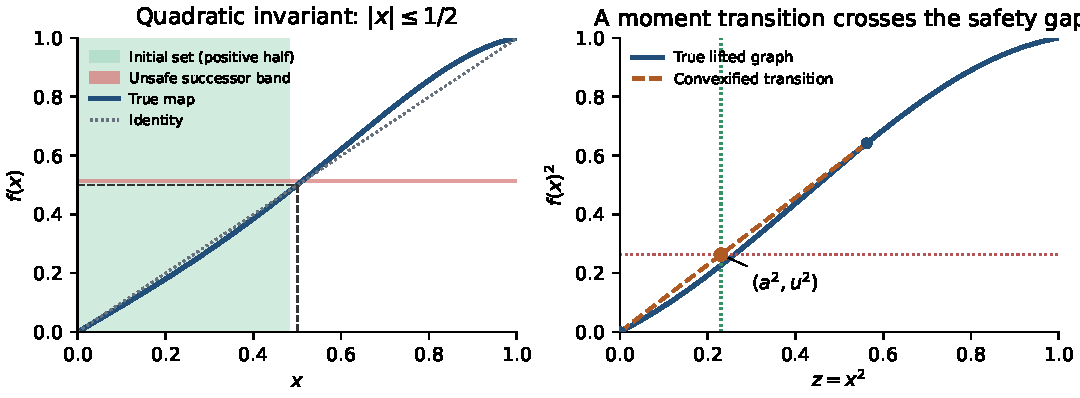
\includegraphics[width=\linewidth]{geometry.pdf}
\end{center}
\vspace{-0.5em}
\textbf{Figure.} Positive half of the symmetric example. In the second-moment plane the chord from $(0,0)$ to $(t^2,f(t)^2)$ contains $(a^2,u^2)$. It connects realizable initial moments to realizable unsafe moments, although the true system keeps $[-1/2,1/2]$ invariant.

\textbf{Verified computation.} \texttt{src/exact\_verify.py} uses only Python's standard-library rational arithmetic. It verifies support and probability constraints, every moment through degree three, the invariant-domain derivative identity, all margins, and the exact factorization and Bernstein coefficients in \eqref{eq:quartic}. Five evidence tests include rejection of a corrupted successor witness and rejection of the same atoms as a degree-four witness. A separate finite-support LP discovery routine recovers a degree-three witness, reconstructs its weights rationally, and repeats exact replay. Its degree-four grid is infeasible; that solver status is \emph{not} the proof of minimum degree. The analytical obstruction plus the explicit quartic certificate establish the degree claim. Plotting is illustrative only. No SOS synthesis run is reported.

\begin{center}\small
\begin{tabular}{@{}p{0.25\linewidth}p{0.31\linewidth}p{0.36\linewidth}@{}}
\toprule
Closest work & Established contribution & Distinction / overlap to assess\\\midrule
Submitted VBC--IBC paper \cite{submission} & Affine convexified transition obstruction; path/scaled duality; rotation separation. & Moment lift extends the obstruction to prescribed degree; exact degree-two versus degree-four example.\\[4pt]
Horvath--Song--Terlaky \cite{horvath} & Theorem 3.1 gives global nonnegative comparisons for affine polyhedral inequalities when successor constraints are concave. & Theorem 1 uses convexification in certificate-value space for arbitrary continuous $B$. Its duality mechanism is classical and should not alone be claimed as the principal novelty.\\[4pt]
Bogomolov et al. \cite{bogomolov} & Convex interpolation discovers template directions that eliminate spurious hybrid counterexamples. & A moment witness identifies spurious transitions that \emph{no added degree-$d$ inequality} can eliminate under global comparison. Models and propagation rules differ.\\[4pt]
Anand et al. \cite{anand} & Path-completeness for soundness and graph ordering via simulation. & Ordering graph structures is distinct from changing global comparisons to sign implications. No switched completeness theorem is claimed here.\\[4pt]
Korda--Henrion--Jones \cite{korda} & Occupation-measure LPs and moment/SOS hierarchies for invariant sets. & The tools are established; the proposed target is nonexistence for an entire finite-degree VBC class with unrestricted finite vector size.\\
\bottomrule
\end{tabular}
\end{center}

\textbf{Domain caveat in the invariance reference.} Horvath et al.'s Theorem 5.1 imposes its comparison only \emph{on the invariant polyhedron}; choosing the zero matrix then proves necessity. It does not imply a comparison on the larger verification domain $X$. This difference is central here. Their Theorem 3.1 does require a global inequality and additional concavity assumptions, consistent with the Jensen regime on page 2.

\newpage
\section{Novelty assessment and the next TAC-level question}
\textbf{What is established in this draft.} Three explicit statements have proofs: a fixed-vector global-comparison characterization, a component-count-independent sufficient degree obstruction, and a parameterized exact $2$--$4$ minimum-degree gap. The first target in Majid's email is met more strongly than requested \emph{within the fixed-anchor class}. These are proposed results with checked finite evidence; they still require independent mathematical and bibliographic review. The present search is targeted, not exhaustive, and does not certify priority or TAC suitability.

\textbf{What the attached publication contributes.} The path-complete closure-certificate paper \cite{pccc} proves a graph soundness characterization for persistence using ordered node-pair relations, with a separate reachability--rank construction. It motivates treating propagation structure as a design choice. It does not supply a fixed-polynomial-degree completeness result, and its relational certificates and persistence specification should not be silently identified with the autonomous safety barriers studied here.

\textbf{Recommended core for a TAC paper.} Develop a \emph{degree-preserving formulation diagnosis}: determine when refinement by more polynomial inequalities can succeed in the convexified feature-transition relation, and when changing the propagation rule is required. The compelling contribution would combine an existence/characterization theorem, exact counterexamples, and a reproducible diagnosis algorithm. The convex-duality theorem and one engineered example alone may be insufficient for TAC.
\begin{enumerate}
\item \textbf{Extend the obstruction through multiple lifted steps.} If $(z_{j-1},z_j)\in F_d$ for $j=1,\ldots,\ell$, with $z_0\in K_{0,d}$ and $z_\ell\in K_{u,d}$, then every forward degree-$d$ VBC obeys $Cz_\ell\leq A^\ell Cz_0\leq0$, a contradiction. The backward proof reverses the inequalities. This is a proved sufficient extension, not yet a complete decision method.
\item \textbf{Seek a converse under robust assumptions.} Establish conditions under which safety of the lifted convex relation yields a finitely faceted invariant feature polyhedron with strict initial inclusion and a fixed unsafe anchor. The existence interpretation on page 2 would then convert it into a VBC. Compactness alone is not asserted to ensure such a finite polyhedron or a terminating algorithm.
\item \textbf{Use counterexamples to select formulations.} First search for exact atomic obstructions at the requested degree. A verified obstruction justifies switching to implication conditions or increasing degree. Otherwise continue synthesis or refine supports; absence of a discovered witness is inconclusive. For fixed $B$, search for a violating probability mixture using Theorem 1, then refine $B$ or change propagation conditions.
\item \textbf{Broaden examples with controlled scope.} The scalar family embeds into $X=[-1,1]\times[-1,1]^q$ with transverse contraction and initial/unsafe product sets. Restricting any degree-three multivariate VBC to the invariant axis $y=0$ inherits the obstruction. Coupling can be introduced via $c(y)$ in the permitted parameter range. These are structured embeddings, not evidence of application-scale performance.
\end{enumerate}

\textbf{Computational safeguards.} A feasible moment-SOS relaxation can contain nonrepresentable pseudomoments; it cannot establish VBC nonexistence without extracted, support-verified measures or another valid analytical argument. Finite-grid LP infeasibility does not exclude witnesses on other supports. Unknown $A$ and unknown $B$ produce bilinear synthesis constraints, so a fixed-$A$ SDP is not a complete search. A positive solver result requires exact replay; failures remain failures of that search. The open parameter result establishes a family, not robustness to arbitrary perturbations of dynamics.

\textbf{Proposed coauthor decision.} Check the proof and scope of Theorems 1--3 and assess the exact degree gap against existing polynomial-template lower bounds. If these survive review, prioritize the robust converse and the multistep diagnosis algorithm before adding switching, control, data-driven guarantees, or persistence specifications.

\newpage
\begin{thebibliography}{9}\small
\bibitem{submission} R. Iraji, V. Murali, and M. Zamani, ``Duality and Complementarity of Vector and Interpolation-Inspired Barrier Certificates for Safety Verification: Toward Reduced Conservatism and Complexity,'' submitted manuscript SCL-D-26-00958, supplied PDF, 2026.
\bibitem{horvath} Z. Horvath, Y. Song, and T. Terlaky, ``Invariance Conditions for Nonlinear Dynamical Systems,'' \href{https://arxiv.org/abs/1607.01107}{arXiv:1607.01107v1}, 2016, Theorems 3.1 and 5.1.
\bibitem{bogomolov} S. Bogomolov, G. Frehse, M. Giacobbe, and T. A. Henzinger, ``Counterexample-guided Refinement of Template Polyhedra,'' TACAS, LNCS 10205, pp. 589--606, 2017. \href{https://doi.org/10.1007/978-3-662-54577-5_34}{doi:10.1007/978-3-662-54577-5\_34}.
\bibitem{anand} M. Anand, R. Jungers, M. Zamani, and F. Allgower, ``On the Completeness and Ordering of Path-Complete Barrier Functions,'' \href{https://arxiv.org/abs/2503.19561}{arXiv:2503.19561v1}, 2025. Comparison is to the supplied version.
\bibitem{korda} M. Korda, D. Henrion, and C. N. Jones, ``Convex Computation of the Maximum Controlled Invariant Set for Polynomial Control Systems,'' SIAM J. Control Optim., vol. 52, no. 5, pp. 2944--2969, 2014. \href{https://doi.org/10.1137/130914565}{doi:10.1137/130914565}.
\bibitem{pccc} R. Iraji, F. Galarza-Jimenez, and M. Zamani, ``Formal Verification of Switched Systems via Path-Complete Closure Certificates,'' supplied IEEE Control Systems Letters accepted author manuscript, 2026. \href{https://doi.org/10.1109/LCSYS.2026.3739034}{doi:10.1109/LCSYS.2026.3739034}.
\bibitem{vector} A. Sogokon, K. Ghorbal, Y. K. Tan, and A. Platzer, ``Vector Barrier Certificates and Comparison Systems,'' FM, LNCS 10951, pp. 418--437, 2018. \href{https://doi.org/10.1007/978-3-319-95582-7_25}{doi:10.1007/978-3-319-95582-7\_25}. Continuous-time foundations; distinct from the discrete-time definition used here.
\bibitem{ibc} M. A. Oumer, V. Murali, A. Trivedi, and M. Zamani, ``Safety Verification of Discrete-Time Systems via Interpolation-Inspired Barrier Certificates,'' IEEE Control Systems Letters, vol. 8, pp. 3183--3188, 2024. \href{https://doi.org/10.1109/LCSYS.2024.3521356}{doi:10.1109/LCSYS.2024.3521356}.
\end{thebibliography}
\end{document}
